\documentclass{article}
% \documentclass[review]{elsarticle}
\usepackage{epsfig}
\usepackage{amsmath}
\usepackage{mathtools}
\usepackage{algorithm}
\usepackage[algo2e,noend]{algorithm2e}
\usepackage[compatible,noend]{algpseudocode}
\usepackage{enumitem}
\usepackage{xspace}
\usepackage[table,xcdraw]{xcolor}
\usepackage{amsfonts}
\usepackage{pifont}
\usepackage{bbding}
\usepackage[english]{babel}
\usepackage{adjustbox}
\usepackage{tikz}
\usetikzlibrary{automata, topaths, calc, positioning, shapes, backgrounds, fit, matrix}
\usepackage{caption}
\usepackage{tabularx}
\usepackage[T1]{fontenc}
\usepackage{natbib}
\usepackage{datatool}
\usepackage{array}
\usepackage{pgfplotstable}
\pgfplotsset{width=7cm,compat=newest}
\usepackage{booktabs}
\usepackage{longtable}
\usepackage{pdflscape}
\usepackage{afterpage}
\usepackage{capt-of}
\usepackage{multirow}
\usepackage{float}
\usepackage[text={15cm,21cm},centering]{geometry}
\usepackage{setspace}
\usepackage{array}
\allowdisplaybreaks
\usepackage{lineno}
\usepackage{tkz-graph}
\usepackage{breqn}
\tikzset{
base/.style = {shape=rectangle, 
                      anchor=center,minimum size=5mm, 
                     align=center,
                     top color=white, ,inner sep=0ex,
                     minimum size=5mm
                     },
    LC11/.style =   {  base,   
                    text width=3em, 
                    bottom color=brown!100,
                    },
    UC11/.style = {     base,    
                    text width=5em, 
                    bottom color=brown!100,
                    align = right,
                },
    LC12/.style =   {  base,   
                    text width=1em, 
                    bottom color=orange!100,
                    },
    UC12/.style = {     base,    
                    text width=2.5em, 
                    bottom color=orange!100,
                },
    LC21/.style =   {  base,   
                    text width=1.5em, 
                    bottom color=brown!100,
                    },
    UC21/.style = {     base,    
                    text width=3.5em, 
                    bottom color=brown!100,
                },
    LC22/.style =   {  base,   
                    text width=4em, 
                    bottom color=blue!100,
                    },
    UC22/.style = {     base,    
                    text width=7em, 
                    bottom color=blue!100,
                    align = left,
                },
    UC221/.style = {     base,    
                    text width=3.5em, 
                    bottom color=blue!100,
                    % color=blue!100,
                    outer xsep=0em,
                    % align = right,
                },
                UC231/.style =   {  base,   
                    text width=1.5em, 
                    bottom color=blue!100,
                    },
    LC23/.style =   {  base,   
                    text width=1.5em, 
                    bottom color=orange!100,
                    },
    UC23/.style = {     base,    
                    text width=2.em, 
                    bottom color=orange!100,
                },
  env/.style      = {base, font=\ttfamily\normalsize},
label/.style   = {base,font=\ttfamily\normalsize, text width = 8em, 
  inner sep=0em, rounded corners=1mm,bottom color=red!80,},
  dummy/.style    = {circle,draw}
}


\newtheorem{theorem}{Theorem}[section]
\newtheorem{lemma}[theorem]{Lemma}
\newtheorem{proposition}[theorem]{Proposition}
\newtheorem{corollary}[theorem]{Corollary}
\newtheorem{definition}[theorem]{Definition}
\newcommand{\pcmaxc}{P$|\mbox{\em cont}|$C$_{\max}$\xspace}
\newcommand{\alns}{adaptive large neighborhood search\xspace}
\newcommand{\Alns}{Adaptive large neighborhood search\xspace}
\newcommand{\F}{$\mathcal{F}$\xspace}
\newcommand{\B}{$\mathcal{B}$\xspace}
\newcommand{\C}{$\mathcal{C}$\xspace}
\newcommand{\Lb}{$\mathcal{L}$\xspace}
\newcommand{\D}{$\mathcal{D}$\xspace}

\renewcommand{\algorithmicforall}{\textbf{for each}}
\SetKwFor{ForEach}{for each}{}{}%
\renewcommand{\algorithmiccomment}[2][1\linewidth]{%
\leavevmode\hfill\makebox[#1][l]{/* \textbf{~#2} */}}
\renewcommand{\algorithmicrequire}{\textbf{Input:}}

\renewcommand{\tabcolsep}{4pt}

\modulolinenumbers[1]
\linenumbers

\oddsidemargin=0.5in
\topmargin=-0.25in
\textwidth=5.5in
\textheight=8.25in

%\journal{European Journal of Operational Research}

%\begin{frontmatter}

		
\title{A GRASP algorithm for the concrete delivery problem. }
\author{Ousmane Ali$^{(1)}$, Jean-Fran\c cois C\^ot\'e$^{(2)}$, Leandro C.~Coelho$^{(3)}$\\
 $(1)$ {\tt nassoma-wattara-ousmane.ali.1@ulaval.ca}\\
 $(2)$ {\tt Jean-Francois.Cote@fsa.ulaval.ca}\\
 $(3)$ {\tt Leandro.Coelho@fsa.ulaval.ca}\\
}

% \date{\today}

\begin{document}
\maketitle
\begin{abstract}
   The concrete delivery problem (CDP) is a combinatorial optimization problem that involves scheduling the delivery of ready-mixed concrete to construction sites while balancing the conflicting goals of minimizing transportation costs and maximizing customer satisfaction. This paper proposes an exact formulation and a heuristic approach based on the Greedy Randomized Adaptive Search Procedure (GRASP) to tackle a new variant of the CDP that incorporates realistic side constraints, such as drivers' working shifts, minimum working time for each driver, and overtime penalties. Additionally, the problem also considers the possibility of customers requiring multiple types of concrete to be delivered within the same time window. The performance of the proposed heuristic is evaluated on real-world and generated CDP instances, and it is compared to another variant to demonstrate its effectiveness.
    
\end{abstract}

% \begin{keywords}
\noindent{\textbf{Keywords:} Vehicle scheduling;  concrete delivery; GRASP; ready-mixed concrete } 
% \end{keywords}

%\end{frontmatter}

\section{Introduction}
\label{sec:intro}
Concrete is a widely used building material in construction projects. It is a perishable product that can be affected by many different factors that impact its quality \citep{sinha_quality_2021} which is crucial for the durability and strength of the final construction.

Concrete comes in two types: ready-mixed concrete (RMC) and site-mixed concrete (SMC). RMC is manufactured in a batch plant and delivered to the construction site, while SMC is produced on-site using raw materials stored on the construction site. Site-mixed concrete can avoid delays caused by road traffic, but it has a slower and more difficult production process, requires storage for mixing materials and equipment, and is suitable for low amounts of concrete. On the other hand, RMC has better quality and benefits from lower production costs \citep{muresan_comparing}. However, to take advantage of these benefits, the batch plant manager must ensure efficient and prompt delivery on the construction site, which may require a fleet of high-cost revolving drum trucks (concrete mixers) to dispatch the ready-mixed concrete.

Concrete delivery under the form of RMC is subject to many operational constraints that make it a challenging problem met in Operations Research and addressed by the Concrete Delivery Problem (CDP). In this paper, we study a variant of the Concrete Delivery Problem to schedule the daily production and dispatching of RMC for a company located in the province of Quebec, Canada. This company operates multiple batching plants with varying production rates, using a fleet of concrete mixers with different capacities. Each plant has its own fleet of trucks, however, the trucks are able to move between plants if necessary. The trucks must return to their home plant at the end of the day. The company owns two types of trucks with different capacities but also has the option to call on an external fleet when needed. They serve construction sites from any of their batch plants, with the first delivery starting at the time specified by the customer. The loading and unloading of a concrete mixer depend on the truck capacity, the loading rate at the plant, and the unloading rate at the construction site. Drivers are allocated based on their daily work schedules. A customer may request several types of concrete to be delivered within the same time window, with no required sequence for the orders, but an order can only start after the completion of the previous order. This constraint generalizes the linked order constraints of \cite{durbin2008or} where some customers place two orders for the same day and request that they are linked (the second order begins only after the first order is completed). The setting of this study is similar to a variant of the Concrete Delivery Problem previously studied in \cite{schmid2009hybrid, schmid2010hybridization}. However, it includes the plant's production rate and driver shift schedule and does not consider unloading instrumentation in contrast to the previous research.
The company uses a centralized dispatcher system to schedule all daily orders, but this system has issues satisfying all daily demands without using an external fleet.
% Also, as per union rules, they assign a truck driver to a delivery task based on his seniority.

According to \cite{blazewicz2019handbook}, the concrete delivery problem combines vehicle routing with scheduling issues to plan routes to deliver concrete from batch plants (depots) to customers' construction sites. Ready-mixed concrete is an on-demand product with a short life cycle from production through end use. It cannot be stored and cannot stay too long in a truck, or it will harden. Hence, concrete mixers must deliver RMC at the planned construction site shortly after its production. RMC production and delivery is described by \cite{tommelein1999just} as an example of a Just-In-Time (JIT) production system in construction. A customer quantity requirement is often greater than the truck size and must be fulfilled by multiple deliveries. In that sense, CDP is like the Vehicle Routing Problem (VRP) with split delivery (VRPSD) \citep{archetti2008split}, except that the same truck may visit a customer more than once. Concrete hardens quickly, so when there are multiple deliveries, they must be done back-to-back or at least close in time to avoid the problem of cold joint, which can reduce the strength and durability of the concrete. Customers request to be served within a specific time window, which can complicate truck-loading schedules when a plant can only load one truck at a time. Similarly, only one truck can unload at a time at a customer location, sometimes leading to concrete mixers queuing and waiting their turn to deliver. Furthermore, with trucks of varied sizes, loading, travel, and unloading times that may be uncertain, the Concrete Delivery Problem is a complex problem to solve and has been proven to be NP-hard \citep{asbach2009analysis,kinable2014concrete}. 

In this paper, we propose a mathematical model and a Greedy Randomized Search Procedure (GRASP) heuristic solution to solve a new variant for the CDP. Our model takes into consideration the working shifts of the drivers and the scheduling of multiple orders within the same time window at a construction site. To the best of our knowledge, this paper is the first that deals with these specific constraints in the context of the CDP.

The rest of the paper is structured as follows: Section \ref{lit_review} provides a literature review of previous work related to the CDP. Section \ref{desc_form} provides a formal description and mathematical model of the problem. In Section \ref{method}, we describe the Greedy Randomized Search Procedure algorithm and the constructive heuristics developed to solve this variant of the CDP. Section \ref{comp_exp}  presents computational experiments to evaluate the proposed approach, and finally, the conclusions are presented in Section \ref{concl}.

\section{Literature review}
\label{lit_review}

A text mining approach by \cite{maghrebi2015text} for reviewing the ready-mixed concrete literature showed that concrete technology and material science are the main core of research in this area. Academic research on concrete batching and delivery began in the late 1990s. \cite{tommelein1999just} described ready-mixed concrete (RMC) as a prototypical example of a Just-In-Time production system in construction and identified two practices for delivering it. One approach is for the customer to haul the product from the batch plant with their concrete mixer, while the other approach is for the batch plant to deliver the concrete directly to the customer's location. This latter approach is the one that has been studied in all related papers found in the literature.

Several works to schedule and dispatch concrete production and delivery have mainly focused on simulation-related methods. These methods can be standalone, such as those used by \cite{zayed2001simulation, wang2001scheduling, tian_simulation_based_2010, panas_simulation_based_2013} and \cite{galic2016simulation}, among others. Alternatively, these methods can be hybridized with optimization techniques, such as those used by \cite{feng2004optimizing, lu2005optimized, feng_integrating_2006}, etc. \cite{wang2001scheduling} developed a simulation model to reveal the effect and value of the concrete mixers' inter-arrival time on the productivity of hired unloading equipment on site. \cite{feng2004optimizing} used a combination of Genetic Algorithm (GA) and simulation process to minimize the total waiting time for trucks at a customer site. The study focused on loading trucks with identical capacities at the same batch plant, with fixed loading and unloading durations. The GA was used to find the best loading sequence of RMC trucks to be assigned to different construction sites. The simulation process determined the loading, arrival, departure, and waiting time of trucks and thus evaluated the cost of each dispatching sequence. They evaluated their method using data from a batch plant in Taiwan with up to nine customers served. \cite{mayteekrieangkrai2015optimized} addressed the same problem with the same data using a bee algorithm (BA) and found better solutions than the GA. \cite{lu2005optimized} used the same combination of GA and simulation to determine the optimal number of concrete mixers to be deployed and an optimal schedule for batching and delivering concrete. Their objective was to minimize the idle time of the site crew due to late concrete deliveries and truck queuing time. In this setting, it was also necessary to deliver a batch of mortar on-site to lubricate the unloading pump before the concrete delivery. As such, the simulation model also included the batching and delivery of mortar. Finding the best RMC truck size was also the purpose of the discrete-event simulation model proposed by \cite{panas_simulation_based_2013}.

In addition to simulation-based methods, several other approaches have been used in the literature to solve the CDP. These include metaheuristics \citep{faria2006distributed, misir2011selection, maghrebi2016sequential, yang2022concrete}, exact methods \citep{yan2007optimal, asbach2009analysis, kinable2014concrete}, matheuristics \citep{schmid2009hybrid, schmid2010hybridization}, Benders Decomposition \citep{maghrebi2014benders}, Column Generation (CG) \citep{maghrebi2014solving, maghrebi2016column}, Lagrangian relaxation \citep{narayanan2015using}, and machine learning approaches such as those used by \cite{graham2006modeling, maghrebi2014exploring, maghrebi2016matching}. \cite{matsatsinis2004towards} designed a decision support system (DSS) for the dynamic routing of both concrete and pumps that may be necessary for some construction sites to aid in the unloading of concrete. The DSS considered the availability of three plants but stipulated that vehicles fulfilling the same order must all load at the same plant. Orders that could not be executed immediately could be postponed for the next day. The routing of the pumps was modelled as a multi-depot vehicle routing problem with time windows. \cite{naso2007genetic} proposed a sequential GA method combined with constructive heuristics to solve another variant of the CDP. In this problem, the plant's production schedule must account for orders for concrete to be delivered to a customer site and orders that customers must pick up themselves. The algorithm first schedules the plant loading operations before scheduling truck deliveries. The authors also developed a non-linear model that minimizes transportation costs, waiting times, outsourced costs, and overtime work. They ran experiments using real-world instances of a concrete supply chain in the Netherlands and found a reduction in the number of requests redirected to external companies. \cite{yan2007optimal} also considered overtime considerations in their paper, which focused on scheduling RMC for one batching plant with two loading docks. The study took into account that overtime wages are paid for factory and construction site operations after 4 PM. They developed a mixed integer programming (MIP) model on a time-space network to minimize travel times and operating costs at both normal and overtime working hours at the plant and the construction sites. They tested the model using real-data consisting of 3 days of operation using a two-stage algorithm. First, they solved the MIP relaxation with CPLEX. Then, they simplified the original model by fixing some decision variables before solving it. The algorithm was found to improve the actual plant operation by 10\%. A time-space network is the key component of the real-time decision support system (DSS) developed by \cite{durbin2008or} to solve a dynamic CDP problem every five minutes. The DSS is able to receive new orders, schedule them on the fly, and handle unexpected events such as plant closures, truck breakdowns, and delays in transportation times. The authors combined the DSS with a Tabu Search (TS) heuristic to warm start CPLEX, which made the model performant enough to solve instances with up to 1,500 loads per day with up to 250 trucks. The DSS also considers the case of a customer who places two orders, with the first being completed before the second starts. Further insights on the real-time planning and monitoring of CDP are available in \cite{garza2021dynamic}. Another variant of the CDP is modeled by \cite{schmid2009hybrid} as an integer multicommodity network flow (MCNF) problem on a time-space network. In this paper, concrete is delivered using a heterogeneous fleet of vehicles, and each plant can load an unlimited number of trucks simultaneously. Some of the trucks have specialized equipment and must arrive first at certain construction sites to assist in unloading the concrete. The objective is to fulfill all orders, minimize the travel cost, and avoid delays between two consecutive unloading operations for an order. The model is typically solved using a matheuristic algorithm that combines the MCNF with a variable neighborhood search (VNS) heuristic. The method can quickly solve large problem instances with more than 60 orders per day without encountering any memory issues. The same problem is addressed by \cite{schmid2010hybridization} who proposed a mixed integer programming (MIP) model combined with a VNS and a very large neighborhood search (VLNS) to develop two matheuristics approaches. Comparisons between both matheuristics and a standalone VNS show that the former methods are much better and suitable for solving larger problem instances. These methods also provide better solutions for small to medium instances than the matheuristic used in \cite{schmid2009hybrid}. A pure VNS approach with the same problem but without the use of instrumentation has been applied by \cite{payr2009optimizing}.

Regarding objectives, most authors have focused on minimizing travel time and delays between consecutive deliveries. However, some authors have been more interested in maximizing customer satisfaction alone. We find these situations in the works of \cite{durbin2008or, kinable2014concrete, kinable2014logic, sulaman2017simulated}. \cite{kinable2014concrete} introduce a general MIP and constraint programming (CP) models of the CDP reflecting the main constraints commonly found in all CDP works: time lag and no overlapping between consecutive deliveries, covering of all customers' demands, delivery time window, and heterogeneous fleet. However, the model did not include constraints limiting the time that concrete may reside in a truck. The authors propose a constructive heuristic that schedules the visits to the customers one by one according to the start time of the visit and the truck capacity. The procedure is invoked multiple times for different permutations of the customer's order which is determined using the steepest descent (SD) local search procedure. One of the paper's main contributions is the creation of the first public test instances for the CDP with up to 50 customers, four batching plants, and 20 concrete mixers. They found the CP model to be highly effective in finding high-quality solutions in relatively little time or improving existing schedules, while the MIP model can be used to compute bounds, as it seems ineffective in solving large problem instances. Finally, the heuristic often yields good solutions in less than a second. A detailed analysis of the MIP model presented in cite{kinable2014concrete}and of two more compact models can be found in the thesis of \cite{hernandez_lopez_study_2020}. In \cite{kinable2014logic}, we found an attempt to solve the previous problem with a Logic Based Benders' approach. \cite{sulaman2017simulated} expand upon the SD heuristic proposed in \cite{kinable2014concrete}, proposing a Simulated Annealing (SA) with a Time-Slot Heuristic (TH). TH mechanism is to look for a slot between existing visits of a truck to schedule a new delivery instead of assigning it to the time slot strictly after the truck's latest assigned delivery. The goal is to reduce the large time gaps that can be present in a schedule created with SD due to ignoring the intermediate available time slots. Experimental results indicated that SATH outperforms SD in speed and solution quality. A generalization of the MIP model of \cite{kinable2014concrete} is addressed in \cite{asbach2009analysis}. This model simultaneously minimizes the total sum of travel costs and the penalty costs for customers with unfulfilled demand. A customer can request that all concrete deliveries come from the same plant or a subset of plants and that a delivery truck belongs to a subset of the vehicle fleet. The MIP model is used in a local search scheme as a black-box solver to reoptimize an incumbent solution in which a neighborhood operator has unfixed some variables. \cite{tzanetos2023systematic} provides an overview of the various methods used in the literature to address the Concrete Delivery Problem and categorizes the problem formulations based on the different concepts used in the literature, such as Integer Programming (IP), time-space network, and job shop model. They also discussed the consistency between industry needs and existing constraints and provided insights into the datasets corresponding to real-world cases, identifying the necessary data for practitioners. 

\section{Problem description}
\label{desc_form}
The focus of this paper is the distribution of ready-mixed concrete from a Canadian company that operates in the greater Montreal area. When a customer places an order, it is received at a central center and then assigned to one of the company's batching plants. These plants produce the concrete and then deliver it to the customer. The problem we are examining involves a set of batching plants, a set of customer orders, and a set of concrete-mixer drivers.

% \subsection*{Batching plants}

The company owns a total of eight batching plants, located in various geographical regions. Each plant has a loading bay that can only accommodate one truck at a time, which leads to trucks lining up. Let $\mathcal{B}$ be the set of batching plants. The plants are heterogeneous, as each plant has its own hourly loading rate, represented by $\tau^l_b$, which affects the duration of the loading process. After the concrete has been loaded, the driver spends $\alpha_b$ minutes adjusting the concrete in the truck before heading to the customer site. A batching plant can serve a construction site as long as the travel time between the two is less than the concrete's lifespan, which is represented by $\Delta$. Each plant has its own assigned fleet of trucks, but it can also borrow trucks from other plants or hire external fleets if necessary.

% \subsection*{Customer orders}

A customer $i$ requests a total of $q_i$ of one or several types of concrete to be delivered to his construction site on a particular day.  We call an order a request for a specific type of concrete. When placing an order $o$, the customer $i$ specifies the required quantity, $q_o$, the desired arrival time of the first concrete mixer, $a_i$, and the unloading rate at their construction site, $\tau^u_i$. If the order requires more concrete than a single truck can carry, multiple deliveries are scheduled. Let $O_i$ be the unordered set of all orders requested by customer $i$. Each element of $O_i$ must be thoroughly delivered before moving on to another order. One element $o$ of $O_i$ must have its first delivery start at $a_i$, while the others can start any time after all deliveries of $o$. Once a plant is chosen to produce a customer's first delivery, it must be the provider of all subsequent deliveries of this customer. To prevent cold joint issues with the concrete, subsequent deliveries must be made just in time, or at least close in time. We define a maximum time lag $\gamma_i$ beyond which no next unloading operation should be allowed. The construction site unloading rate and the quantity to unload give the time necessary to discharge a truckload. $\mathcal{C}$ is the set of construction sites (customers) with a planned delivery for the day. $\mathcal{O}$ is the set of all requested orders. 

% \subsection*{Drivers}

The company has two types of concrete mixer trucks with capacities of 8 and 12 cubic meters. Each driver $k$ is assigned to a specific batching plant and is responsible for driving a truck with a specific capacity $Q_k$. The set of drivers is represented by $K =\cup_{b \in \mathcal{B}}K_b $, $K_b$ being the set of drivers scheduled to start their shift at the batching plant $b$. $t_{ij}$ is the known time to travel between any two locations $i$ and $j$.
A scheduled driver $k$ is required to begin their shift at $H_k$, work for a minimum of $M_T$ hours and a maximum of $N_T$ hours during regular working hours, with the possibility of overtime of up to $O_T$ hours. %Let the continuous variable $WT_k$ be the working time of each driver $k$ during a day ($WT_k \leq O_T$). $\Gamma_1$ and $\Gamma_2$ are the incurred penalties when a driver works less than $M_t$ and more than $N_t$. 

A driver typically loads RMC at their assigned batching plant, but may also be required to drive to and load at other plants if needed. Batching plant produces concrete on-demand with recipes specific to each customer. This means that a truck cannot hold orders for more than one customer, even if there is spare capacity. To fulfill multiple orders, a driver must refill at a plant between deliveries. After unloading the RMC, a driver takes $\beta_k$ minutes to clean the concrete mixer before travelling to his next loading plant. %When assigning drivers to deliveries, the company prioritizes employees with the highest seniority.

% \subsection*{Model}

A solution to the problem involves making decisions about truck loading schedules, driver assignments to different deliveries, and truck arrival times at construction sites for unloading. For a batching plant, the decision involves choosing which driver to load, when to load them, and which construction site they should deliver to. For a driver, the decision involves determining the sequence of loading depots and delivery sites. And for a construction site, the decision involves determining the arrival times of all scheduled deliveries for the day.

We now present a formal definition of our problem. Let $n_o$ be the number of deliveries needed to fulfill order $o$. $n_o$ is not known in advance, as we use a fleet of trucks with various capacities. However, we can compute its lower ($n_o^{min}$) and upper ($n_o^{max}$) bounds using the capacities of the highest ($Q_{max}$) and smallest ($Q_{min}$) available trucks. The lower bound is the number of deliveries needed if we only use trucks of capacity $Q_{max}$, while the upper bound is the number of deliveries needed if we only use trucks of capacity $Q_{min}$. 

\begin{alignat}{3}
    \label{mod:c1}
       \left\lceil \frac{q_o}{Q_{max}} \right\rceil \leq n_o \leq \left\lceil \frac{q_o}{Q_{min}} \right\rceil  & \text{ } & 
 \forall  o \in \mathcal{O}.
\end{alignat}

Let $d^j_{o}$ be the $j_{th}$ visit with load $q^j_{o}$ for order $o$. We represent the delivery of order $o$ by the visits to the ordered set of nodes $\mathcal{D}_o= \left(d^0_{o},d^1_{o},\cdots, d^{n_o}_{o}\right)$. We represent the deliveries of customer $i$ by the ordered set $\mathcal{D}_i= (\mathcal{D}_{o_1}, \mathcal{D}_{o_2},\cdots,\mathcal{D}_{o_{|O_i|}})$, where $o_r$ is the $rth$ order delivered. We will refer to $d \in \mathcal{D}_i$ ($d \in \mathcal{D}_o$) as the $dth$ potential delivery of customer $i$ (order $o$). $\mathcal{D}=\bigcup_{i\in \mathcal{C}} \mathcal{D}_i$ is the union of all delivery nodes. 

We represent each plant $b$ by the ordered set $L_b=\{L_{b,1}, L_{b,2},\cdots, L_{b,n(b)}\}$ of loading docks nodes, with $n(b)$ being the number of delivery nodes at a maximal travel time of $\Delta$ of $b$. We will refer to $L_{b,l}$ or  $l \in L_b$  as the $lth$ potential loading operation at $b$. $\mathcal{L}=\bigcup_{b\in B} L_b$ is the union of all loading docks. 

Each driver leaves and returns to his home plant each day. We represent a driver $k$ home plant's with a starting $s_k$ and ending $e_k$ depot. $S$ and $E$ are respectively the sets of starting and ending depot.

We define our problem on a complete directed graph where $V=\{ S \cup \mathcal{L} \cup \mathcal{D} \cup E\}$ is the set of nodes. The arc sets are $A =  \{(i,j,k) \hspace*{1mm} \vert \hspace*{1mm} i, j \in V \hspace{1mm} k\in K \}$, and $A^D = \{(i,j) \hspace*{1mm} \vert \hspace*{1mm} i, j \in \mathcal{D} \hspace{1mm} \}$. 
$A$ corresponds to allowed movements of drivers from node $i$ to node $j$. For each driver $k$, the allowed movements are the following:
\begin{itemize}
    \item From the starting depot $s_k$ to a loading dock $l \in \mathcal{L}$ or to the ending depot $e_k$.
    \item From a loading dock $l \in \mathcal{L}$ to a delivery node $d \in \mathcal{D}$.
    \item From a delivery node  $d \in \mathcal{D}$ to a loading dock $l \in \mathcal{L}$ or to the ending depot $e_k$.
\end{itemize}

For a customer $c$, arcs in $A^D$ link consecutive delivery nodes of the same order   $\lbrace (i,j)\in \mathcal{D}_o, o \in \mathcal{O}_c, i < j  \rbrace$, and pair of delivery nodes of two different orders $ \lbrace (i,d^{0}_{o_2}),  i \in \mathcal{D}_{o_1}, i \geq n^{min}_{o_1}, o_1, o_2 \in \mathcal{O}_c, o_1 \neq o_2 \rbrace $.

$\delta^{+}(i) = \{(i, j,k) \in A \}$, and $\delta^{-}(i) = \{(j, i,k) \in A \}$ are the outcoming and incoming arc sets of any node $i \in V$. Similarly, $\delta^{+}_D(i) = \{(i, j)  \in A^D\}$, and $\delta^{-}_D(i) = \{(j, i) \in A^D \}$ are the outcoming and incoming arc sets of delivery node $i \in \mathcal{D}$.

Let the binary variable $x^{k}_{ij}$ be $1$ if driver $k$ travels from node $i$ to $j$. Binary variable $y_i$ equals $1$ if customer $i$ is completely served. $v_i$ is the start of the loading (unloading) operation at node $i \in L \cup D$. $w_i$ is the end of the loading (unloading) operation at node $i \in L\cup D$. The binary variable $u_{i,j}$ equals $1$ if delivery node $j$ is served just after delivery $i$.  Binary variable $\sigma_{ib}$ equals 1 if customer $i$ orders' are loaded from plant $b$. % Binary variable $u_{o_{1},o_{2}}$ equals $1$ if order $o_{2}$ is served directly after order $o_{1}$. Binary variables $z_{o,d}$ ($z_{i,d}$) indicates whether or not delivery $d \in  \mathcal{D}_o$ ($d \in  \mathcal{D}_i$) is supposed to be executed.

A driver $k$ leaves his starting node exactly once a day and travels to either a loading dock or his ending node. When loading at a loading dock $i$, he takes some time to adjust the concrete in the truck before travelling to delivery node $j$ to unload. The loading operation duration depends on the plant loading rate and the quantity $q^k_j$ of RMC to load towards $j$. After completing his last unloading operation of the day, he returns to his end node.

\begin{alignat}{3}
\label{mod:c2} \sum_{j \in \delta^{+}(s_k) }{x^k_{s_kj}} = 1 & \text{ } &\forall k \in K \\
\label{mod:c3}   v_j \geq  w_i + \alpha_{i} + t_{ij} - M(1-x^{k}_{ij}) & \text{ }& \forall i \in \mathcal{L}, j \in \mathcal{D},  k \in K \\
\label{mod:c4}  w_{i} \geq v_{i}  + \frac{q^k_j}{\tau^l_b} -M(1- x^{k}_{ij}) &  \hspace{5mm} &\forall  b \in \mathcal{B},  i \in L_{b}, j \in \mathcal{D}, k \in K \\
\label{mod:c5} \sum_{j \in \delta^{-}(e_k)}{x^k_{je_k}} = 1 & \text{ }   &  \forall k \in K
\end{alignat}

Constraints (\ref{mod:c4}) ensure that two trucks cannot be loaded at the same time in a plant.

\begin{alignat}{3}
    \label{mod:c6}       w_{l-1} \leq v_{l} & \hspace{5mm} &\forall  b \in B,  l \in L_{b}, l \geq 1 
\end{alignat}

After completing a delivery  at node $i$, a driver must clean the truck, and travel to the next loading depot or end node. The unloading service depends on the construction site's rate and the received quantity. Unloading operations must finish $\Delta$ minutes after the begin of loading.
\begin{alignat}{3}
    \label{mod:c7}     v_j \geq  w_i + \beta_{k} + t_{ij} - M\left(1-x^{k}_{ij}\right) & \text{ }& \forall i \in \mathcal{D}, j \in \mathcal{L} \cup \{e_k\},   k \in K \\
    \label{mod:c8}          w_{j} \geq v_{j}  + {  \frac{q^k_j}{\tau^u_c} -M\left(1- x^{k}_{ij}\right) } & \text{ }&  \forall c \in  \mathcal{C}, j \in \mathcal{D}_{c}, i \in \mathcal{L},  k \in K \\
    \label{mod:c31}          w_{j} \leq v_{i}  + \Delta + M\left(1- x^{k}_{ij}\right)&  \text{ }&  \forall c \in  \mathcal{C}, j \in \mathcal{D}_{c}, i \in \mathcal{L},  k \in K
    % \label{mod:c31}      w_{d-1}  \leq v_{d} & \hspace{5mm} & \forall i \in \mathcal{C}, o \in O_i, d \in \mathcal{D}_{o}, d \geq 1 \\
    % \label{mod:c10}      z_{o,d} \leq z_{o,d-1} & \hspace{5mm} & \forall i \in \mathcal{C}, o \in O_i, d \in \mathcal{D}_{o}, d \geq 1\\
    % \label{mod:c11}  v_{d} - w_{d-1} \leq \gamma_i   & \hspace{5mm}&  \forall i \in \mathcal{C}, o \in O_i, d \in \mathcal{D}_{o}, d \geq 1
\end{alignat}

The first service of any customer $i$ has to start at the due time $a_i$. Let $g_i$ be the gap between the due time and the start of first service at $i$. This first service may be performed at the first delivery node of any order $\in O_i$. Constraints (\ref{mod:c11}--\ref{mod:c13}) are used to find the delivery sequence of the first delivery node of all orders $\in \mathcal{O}_i$.

\begin{alignat}{3}
    \label{mod:c9}   v_{d^0_{o}} \geq a_i & & \forall  i \in \mathcal{C}, \forall o \in \mathcal{O}_i\\
    \label{mod:c10}  g_{i} \geq v_{d} - a_i - M\left(  \sum_{ j \in \delta^{-}_{D}(d)  }{u_{j,d}}\right) & & \forall  i \in \mathcal{C}, \forall o_1 \in \mathcal{O}_i, d=d^0_{o_1} \\
    \label{mod:c11}   \sum_{ \substack{o_1 \in \mathcal{O}_i }}{ \sum_{ j \in \delta^{-}_{D}(d^0_{o_1})}}{u_{j,d^0_{o_1} } } = |\mathcal{O}_i|-1 & \text{ }& \forall  i \in \mathcal{C},|\mathcal{O}_i| > 1 \\
    \label{mod:c12}   \sum_{ \substack{o_1 \in \mathcal{O}_i }}\sum_{ j \in \delta^{+}_{D}(d^0_{o_1})}{u_{d^0_{o_1},j } } = |\mathcal{O}_i|-1 & \text{ }& \forall  i \in \mathcal{C}, |\mathcal{O}_i| > 1 \\
    \label{mod:c13}  \hspace{3mm} \smashoperator{ \sum_{ j \in \delta^{+}_{D}(d^0_{o_1})}}{u_{d^0_{o_1},j } } \leq 1, \hspace{2mm} \smashoperator{ \sum_{ j \in \delta^{-}_{D}(d^0_{o_1})}}{u_{j,d^0_{o_1} } } \leq 1, \hspace{2mm} \smashoperator{ \sum_{ j \in \delta^{+}_{D}(d^0_{o_1})}}{u_{d^0_{o_1},j } } +\smashoperator{ \sum_{ j \in \delta^{-}_{D}(d^0_{o_1})}}{u_{j,d^0_{o_1} } } \geq1         & \text{ }& \forall  i \in \mathcal{C}, \forall o_1 \in \mathcal{O}_i
\end{alignat}

For a customer, an order must be completed before starting another. Constraints (\ref{mod:c14}--\ref{mod:c15}) enforce the precedence constraints between the last delivery of an order and the first delivery of the subsequent order. 

\begin{alignat}{3}
  \label{mod:c14} & v_{d^0_{o_2}} \geq w_j - M(1- u_{j,d^0_{o_2}}) & \text{} & \forall i \in \mathcal{C}, \forall o_1, o_2 \in O_i, j \in \mathcal{D}_{o_1}, (j,d^0_{o_2}) \in \delta_{D}^{-}(d^0_{o_2})  \\
  \label{mod:c15} &  v_{d^0_{o_2}}  \leq  w_j + \gamma_i + M(1- u_{j,d^0_{o_2}}) & \hspace{1mm} & \forall i \in \mathcal{C}, \forall o_1, o_2 \in O_i, j \in \mathcal{D}_{o_1}, (j,d^0_{o_2}) \in \delta_{D}^{-}(d^0_{o_2}) 
%   \label{mod:c12} & v_{j} \geq w_d - M(1- u_{d,j}) & \text{} & \forall i \in \mathcal{C}, \forall o_1 \in O_i, d= d_{o_1,0}, j \in \mathcal{D}_{i}, j \neq  d\\
%   \label{mod:c112} &  v_{j}  \leq  w_d + \gamma_i + M(1- u_{d,j}) & \text{ } & \forall i \in \mathcal{C}, j \in \mathcal{D}_{i}, o_1 \in O_i, d= d_{o_1,0},    j \neq  d\\
%   \label{mod:c112} &  \smashoperator{\sum \limits_{j \in \mathcal{D}_i, j\neq d}}{u_{d,j}} \leq 1 & \text{ } & \forall i \in \mathcal{C}, o \in O_i,  d = d_{o,0} \\
%   \label{mod:c113} &  \smashoperator{\sum \limits_{j \in \mathcal{D}_i, j\neq d}}{u_{j,d}} \leq 1 & \text{ } & \forall i \in \mathcal{C}, o \in O_i,  d = d_{o,0} \\
%   \label{mod:c111} &  \smashoperator{\sum \limits_{j \in \mathcal{D}_i, j\neq d}}{u_{d,j}}+ \smashoperator{\sum_{j \in \mathcal{D}_i, j\neq d}}{u_{j,d}} \geq 1 & \text{ } & \forall i \in \mathcal{C}, o \in O_i,  d = d_{o,0} 
\end{alignat}

Constraints (\ref{mod:c29}--\ref{mod:c30}) enforce the precedence constraints between two consecutive delivery nodes of the same order.

\begin{alignat}{3}
\label{mod:c29}   &   u_{j-1,j} \geq u_{j,j+1} & \hspace{5mm} & \forall i \in \mathcal{C}, \forall o \in O_i,  j \in \mathcal{D}_{o}, 1 \leq j \leq n_o-1\\
  \label{mod:c30} &  u_{j-1,j} \geq \sum_{l \in \mathcal{L}}{x_{lj}} & \text{} & \forall i \in \mathcal{C}, \forall o \in O_i, j \in \mathcal{D}_{o}, j \geq 1 
\end{alignat}

Constraints (\ref{mod:c17}--\ref{mod:c18}) state that it is not possible for two trucks serving consecutive deliveries to be unloaded at the same time and there is a maximum time lag between them.

\begin{alignat}{3}
  \label{mod:c17} & v_{j} \geq w_{j-1} - M(1- u_{j-1,j}) & \text{} & \forall i \in \mathcal{C}, \forall o \in O_i, j \in \mathcal{D}_{o}, j \geq 1 \\
  \label{mod:c18} &  v_{j}  \leq  w_{j-1} + \gamma_i + M(1- u_{j-1,j}) & \text{ } & \forall i \in \mathcal{C}, \forall o \in O_i, j \in \mathcal{D}_{o}, j \geq 1
\end{alignat}

With constraints (\ref{mod:c19}) and (\ref{mod:c20}), we respectively impose that the cumulative capacity of all concrete mixers serving an order and a customer may exceed the required quantities.

\begin{alignat}{1}
    \label{mod:c19} \sum_{d \in D_o}\sum_{k \in K}{q^k} \sum_{j \in \mathcal{L}}{x^k_{jd}}\geq q_o, \forall o \in \mathcal{O} \\
    \label{mod:c20} \sum_{d \in D_i}\sum_{k \in K}{q^k} \sum_{j \in \mathcal{L}}{x^k_{jd}}\geq q_i, \forall i \in \mathcal{C}
\end{alignat}

Constraints (\ref{mod:c21}) and (\ref{mod:c22}) impose that a loading or delivery node may only be visited once by one driver. Constraints (\ref{mod:c23}) and (\ref{mod:c24}) are degree constraints.

\begin{alignat}{3}
\label{mod:c21} &  \sum_{k \in K}\sum_{j \in \mathcal{D}}{x^{k}_{ij} \leq 1} & \text{ } & i \in \mathcal{L}\\
  \label{mod:c22}  &  \sum_{k \in K}\sum_{i \in \mathcal{L}}{x^{k}_{ij} \leq 1} & \text{ } & j \in \mathcal{D} \\
  \label{mod:c23}  &  \sum_{k \in K}\sum_{i \in \mathcal{L}}{x^{k}_{ij} } =  \sum_{k \in K}\sum_{i \in \mathcal{L}}{x^{k}_{ji} } & \text{ } & j \in \mathcal{D} \\
  \label{mod:c24}  &  \sum_{k \in K}\sum_{i \in \mathcal{D}}{x^{k}_{ij} } =  \sum_{k \in K}\sum_{i \in \mathcal{D}}{x^{k}_{ji} } & \text{ } & j \in \mathcal{L}
\end{alignat}

 Constraints (\ref{mod:c25}) and (\ref{mod:c26}) impose that all orders of customer $i$ must be loaded from the same plant.
 
\begin{alignat}{2}
    \label{mod:c25} & \sum_{k \in K} \sum_{l \in \mathcal{L}_b} \sum_{d \in \mathcal{D}}{x^k_{ld}} \leq M*\sigma_{i, b} & \forall i \in \mathcal{C}, b \in \mathcal{B} \\
    \label{mod:c26} & \sum_{b \in \mathcal{B}} \sigma_{i, b} \leq 1 & \text{ } \forall i \in \mathcal{C}, b \in \mathcal{B} 
\end{alignat}

Let $w^1_k$ be the binary variables indicating if the driver $k$ has reached the minimum number of hours worked in the day. $w^2_k$ is a continuous variable indicating the gap between the driver working time and the normal working time.

\begin{alignat}{3}
    \label{mod:c27}  M_T*w^1_k \leq v_{e_k} - H_k & \hspace{5mm} &\forall k \in K \\
    \label{mod:c28}  w^2_k \geq (v_{e_k} - H_k) - N_T & \hspace{5mm} &\forall k \in K.
\end{alignat}

The objective function (\ref{mod:obj}) minimizes the travelled distance, the penalty costs incurred when customers' demands are not fully satisfied, the lateness of each customer first delivery, the number of drivers who work under the minimum working time and the total overtime cost when drivers work beyond their scheduled hours.
%The objective function (\ref{mod:obj}) is designed to minimize multiple factors that impact the overall cost and efficiency of the concrete delivery process. These factors include: The total traveled distance, which represents the fuel consumption and wear and tear on the delivery vehicles. The penalty costs $\beta_1$, which are incurred when customers' demands are not fully satisfied.The lateness of each customer's first delivery, which can impact customer satisfaction and lead to additional penalty costs.The number of drivers who work under the minimum working time, which can lead to increased labor costs and decreased productivity.The total overtime cost, which is incurred when drivers work beyond their scheduled hours.All these factors are taken into consideration in the objective function to minimize the cost and maximize the satisfaction of the customers.
\begin{align}
\label{mod:obj}
\hspace{-20mm}
    \begin{split}
      \min  \smashoperator{\sum_{k \in K}} \sum_{ \substack{i \in \mathcal{L}} } \sum_{ j \in \delta^{+}{(i)} } {t_{ij}x^{k}_{ij}} + 
      \sum_{k \in K} \sum_{ \substack{i \in \mathcal{D}}} \sum_{j \in \delta^{+}{(i)} } {t_{ij}x^{k}_{ij}} + 
      \smashoperator{\sum_{ i \in C}}{ \beta_1 \left(1-y_i\right)} \hspace{-0mm} \\ +
      \beta_2 \smashoperator{ \sum_{i \in \mathcal{C} } } { g_i  } 
    %   + \beta_3 \smashoperator{\sum_{i \in \mathcal{C}}}{  {\sum_{d \in D_i}}{\left(v_d - w_{d-1} - \gamma_i\right)} } 
      +  \sum_{k \in K}{\beta_3* w^{1}_k } + \beta_4 *{ w^{2}_k }
    \end{split}
\end{align}

\iffalse
graphe: G=(V,A)
arc between origin depot, depot
arc between depot delivery node
arc between delivery node -> depot
arc between delivery node -> origin depot



Let $SLT^{bk}_{j}$ and $ELT^{bk}_{j}$ be the start and end loading time of driver $k$ at plant $b$. $SUT_{j}$, $EUT_{j}$ be the start and end unloading time. $LTS^{bk}_{j}=\left[ SLT^{bk}_{j}, ELT^{bk}_{j} \right] $, and $UTS^{bk}_{j}=\left[ SUT^{bk}_{j}, EUT^{bk}_{j} \right]$ stand for the loading  and unloading operations timeslots. $AT_{j}$ is the arrival time of a driver at the node location.

\begin{alignat}{2}
    \label{eq:ELT}  ELT^{bk}_{j} &= SLT^{bk}_{j}+ LD^b_{j}\\
    \label{eq:S}         EUT_{j} & = SUT_{j} + UD_{j}
\end{alignat}

For each delivery node $j$, we define an expected delivery time $EDT_{j}$ of unloading operation, the driver waiting duration $W^k_{j}$, and the node waiting time $W_{j}$.


\begin{alignat}{3}
    \label{eq:ES} EDT_{d^{p^l}_{ij}} &=
          \begin{cases}
            a_i & \text{if $j=0$, $l=0$}\\
            E_{d^{p^l}_{ij-1}} & \text{ $j \geq 1$}\\
            E_{d^{p^{l-1}}_{in^{p^{l-1}}_i}}  & 
          \end{cases} &  \\
    \label{eq:Wd} W^k_{d^p_{ij}} &= \max\{0, SUT_{d^p_{ij}} - AT_{d^p_{ij}}\} & \\
    \label{eq:Wc} W_{d^p_{ij}} & = \max\{0, AT_{d^p_{ij}} - EDT_{d^p_{ij}}- \lambda_i \} &
\end{alignat}

\fi

\paragraph*{}
Let us consider the solution of a small instance of our problem illustrated in Figures~\ref{fig_Example} and \ref{fig:ganttExample}. Two batching plants $B_1$ and $B_2$ with three drivers serve two construction sites. Customer $C_1$ requests one order of $q^1_1=12$ m$^3$. Customer $C_2$ requests three orders of $q^1_2=3$, $q^2_2=11$, and $q^3_2=1$ m$^3$ of three different types of concrete. $B_1$ has two drivers ($D_1$, $D_2$) using concrete mixers of capacity 8 m$^3$, and $B_2$ has $D_3$ of capacity 12 m$^3$. Figure~\ref{fig_Example} depicts the concrete mixers flow in the network. We schedule $D_1$ and $D_2$ to respectively deliver 8 and 4 m$^3$ to $C_1$. We select $o^2_2$ as the first order of $C_2$ to deliver. $D_3$ travels to $B_1$ to load $q^2_2$, then visits $C_2$ before returning to his home plant. Meanwhile, after their first trip,  $D_1$ and $D_2$ deliver the remaining orders of $C_2$.

Figure~\ref{fig:ganttExample} shows the sequence of loading and unloading operations. The first deliveries of $C_1$ and $C_2$ are timely and there is no gap between the two deliveries received by $C_1$. There is a delay between the end of the first delivery and the start of the second delivery of $C_2$, however, it is less than the maximal time lag of 20 minutes defined for this example.


\begin{figure}[!ht]
    % \caption{Solution of an instance with two plants, two construction sites, four orders, and three drivers.}
    \vspace*{-10mm}

    \centering
    \begin{adjustbox}{max width=0.85\textwidth}
      
  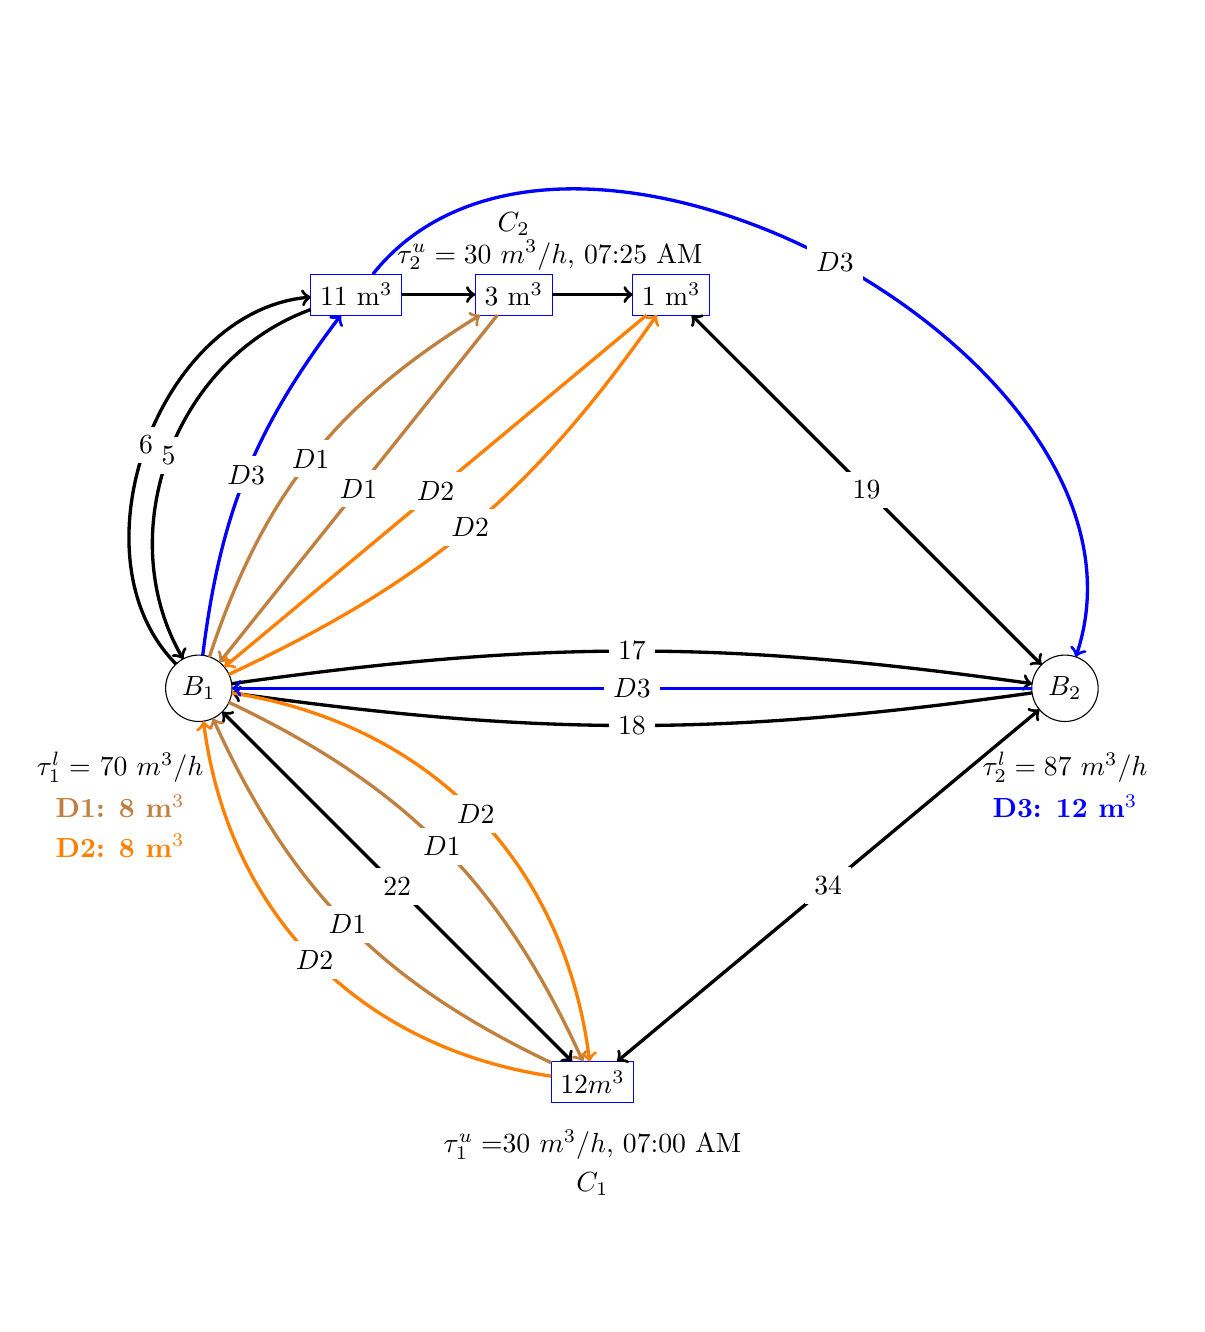
\begin{tikzpicture}
    \SetUpEdge[lw = 1.2pt,
        labelcolor = white,
        % labelstyle = {draw}
    ]
    \tikzstyle{LabelStyle}=[fill=white]

    \SetGraphUnit{5}
    \GraphInit[vstyle=Normal]
    \tikzset{VertexStyle/.style = {shape = circle,text = black,minimum size = 24 pt,draw = black}}
    \Vertex[L={$B_1$}]{D1}
    \tikzset{VertexStyle/.style = {shape = circle,text = black,minimum size = 10 pt,draw = blue}}
    \tikzset{VertexStyle/.style = {shape = rectangle,text = black,minimum size = 10 pt,draw = blue}}
    \Vertex[x=2,y=5,L={11 m$^3$}]{C21}
    \EA[unit=2.0,L={3 m$^3$}](C21){C22}
    \EA[unit=2.0,L={1 m$^3$}](C22){C23}
    \tikzset{VertexStyle/.style = {shape = rectangle,text = black,minimum size = 10 pt,draw = blue}}
    \SOEA[L={$12m^3$}](D1){C1}
    \tikzset{VertexStyle/.style = {shape = circle,text = black,minimum size = 24 pt,draw = black}}
    \SOEA[L={$B_2$}](C23){D2}
    % %  \SetVertexArt
    \tikzset{VertexStyle/.style = {shape = circle,text = black,minimum size = 10 pt}}
    \SO[unit=0.8,L={$\tau^u_1=$30 $m^3/h$, 07:00 AM}](C1){tau1}
    \SO[unit=0.5,L={\textbf{$C_1$} }](tau1){o1}
    
    \NO[unit=0.9,L={\textbf{$C_2$}}](C22){C2}
    \SOEA[unit=0.4,L={\textcolor{white}{  } $\tau^u_2=30$ $m^3/h$, 07:25 AM}](C2){tau2}

    \tikzset{VertexStyle/.style = {shape = rectangle,text = black,minimum size = 10 pt}}
    \SOWE[unit=1.,L={$\tau^l_1=$ 70 $m^3/h$}](D1){cap1}
    \SO[unit=0.5,L={\textbf{\textcolor{brown}{D1: 8 m$^3$}}}](cap1){driver11}
    \SO[unit=0.5,L={\textbf{\textcolor{orange}{D2: 8 m$^3$}}}](driver11){driver12}
    \SO[unit=1,L={$\tau^l_2= 87$ $m^3/h$}](D2){cap2}
    \SO[unit=0.5,L={\textbf{\textcolor{blue}{D3: 12 m$^3$}}}](cap2){driver2}
    %%%%%%% Edge
    \tikzset{EdgeStyle/.style={->}}
    \Edge[](C21)(C22)
    \Edge[](C22)(C23)
    \tikzset{EdgeStyle/.style={<->,bend left=0}}
    \Edge[label=$22$](D1)(C1)
    \tikzset{EdgeStyle/.style={<->}}
    \Edge[label=$19$](D2)(C23)
    \Edge[label=$34$](D2)(C1)
    \tikzset{EdgeStyle/.style={->}}
    \tikzset{EdgeStyle/.append style = {bend left = 8}}
    \Edge[label=$17$](D1)(D2)
    \Edge[label=$18$](D2)(D1)
    \tikzset{EdgeStyle/.append style = {bend left = 65}}
    \Edge[label=$6$](D1)(C21)
    \tikzset{EdgeStyle/.append style = {bend right = 50}}
    \Edge[label=$5$](C21)(D1)
    \tikzset{EdgeStyle/.style = {->,bend left = 20,draw=brown}}
    \Edge[label=$D1$](D1)(C1)
    \Edge[label=$D1$](C1)(D1)
    \tikzset{EdgeStyle/.style = {->,bend left = 37,draw=orange}}
    \Edge[label=$D2$](C1)(D1)
    \Edge[label=$D2$](D1)(C1)

    \tikzset{EdgeStyle/.style = {->,bend left= 20,draw=brown}}
    \Edge[label=$D1$](D1)(C22)
    \tikzset{EdgeStyle/.style = {->,bend left= 0,draw=brown}}
    \Edge[label=$D1$](C22)(D1)
    
    \tikzset{EdgeStyle/.style = {->,bend left = 0,draw=orange}}
    \Edge[label=$D2$](C23)(D1)
    \tikzset{EdgeStyle/.style = {->,bend left = -15,draw=orange}}
    \Edge[label=$D2$](D1)(C23)
    

    \tikzset{EdgeStyle/.style = {->,,draw=blue}}
    \Edge[label=$D3$](D2)(D1)
    \tikzset{EdgeStyle/.style = {->,bend left = 15,draw=blue}}
    \Edge[label=$D3$](D1)(C21)
    \tikzset{EdgeStyle/.style = {->,bend left = 80,draw=blue}}
    \Edge[label=$D3$](C21)(D2)
    \end{tikzpicture}
    \end{adjustbox}
    \vspace*{-10mm}
    % }
    \caption{Solution of an instance with two plants, two construction sites, four orders, and three drivers.}
    \label{fig_Example}

\end{figure}

\begin{figure}[!htb]
    \centering
    
    \vspace*{-0mm}
    \begin{adjustbox}{max width=0.85\textwidth}
        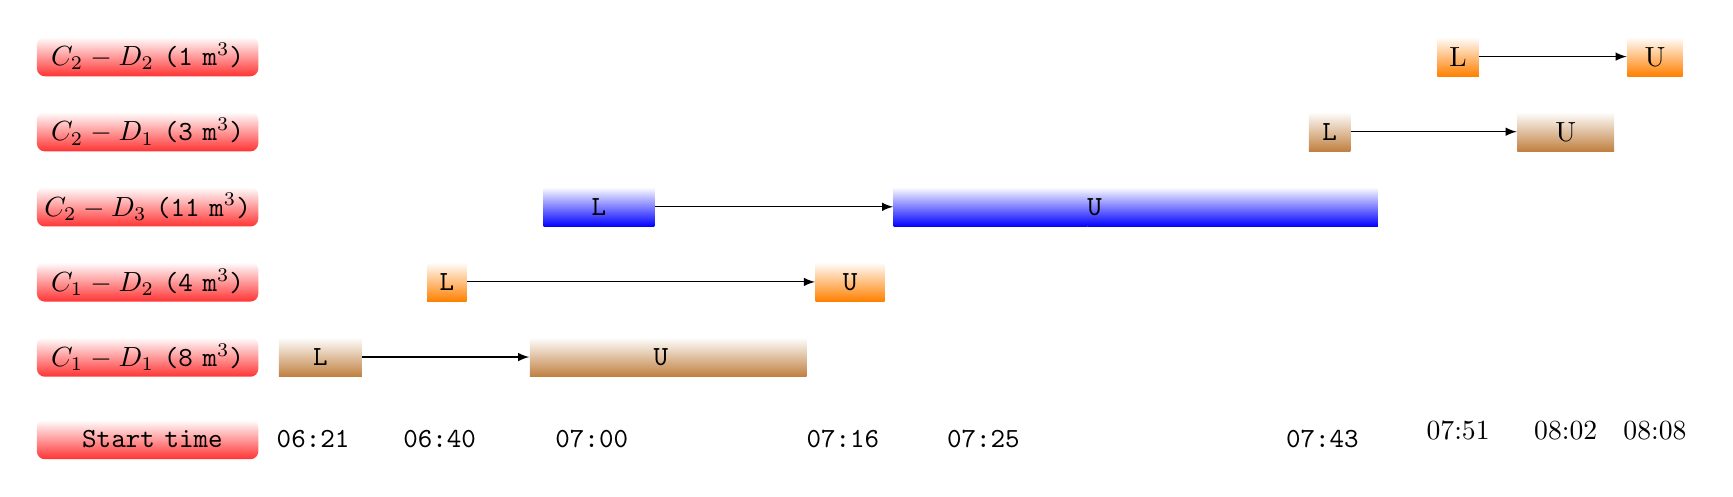
\begin{tikzpicture}[-latex]
            \matrix (chart)
            [
            matrix of nodes, nodes in empty cells,
            column sep      = 0em,
            row sep         = 3ex,
            column 1/.style = {nodes={label}},    column 2/.style = {},       column 3/.style = {nodes={env}},      column 4/.style = {nodes={env}},         column 5/.style = {nodes={env}},         column 6/.style = {nodes={env}},           column 7/.style = {nodes={env}},           column 8/.style = {nodes={env}},           column 9/.style = {nodes={env}},           column 10/.style = {nodes={env}},         column 11/.style = {nodes={env}},           column 12/.style = {nodes={env}},    column 13/.style = {nodes={env}}
            ]
            {
            $C_2-D_2$ (1 m$^3$) &
            &   &   &   &   &   &   &   &   &   &   &   &            |[LC23]| L &            &       &     |[UC23]| U \\
            $C_2-D_1$ (3 m$^3$) &           &      &        &        &           &            &            &
            &
            &
            &
            |[LC21]| L &
            &
            &
            &
            |[UC21]| U &
            \\
            $C_2-D_3$ (11 m$^3$) &
            &
            &
            &
            &
            &
            |[LC22]| L &
            &
            &
            |[UC22]| &
            |[UC22]|U  &
            |[UC221]|  &
            &
            &
            &
            &
            \\
            $C_1-D_2$ (4 m$^3$) &
            &
            &
            &
            |[LC12]| L &
            &
            &
            &
            |[UC12]| U &
            &
            &
            &
            &
            &
            &
            &
            \\
            $C_1-D_1$ (8 m$^3$) &
            &
            |[LC11]| L &
            &
            &
            &
            |[UC11]|U &
            |[UC11]| &
            &
            &
            &
            &
            &
            &
            &
            &
            \\
            \vspace*{-10em}
            Start time &&
            06:21 &
            &
            06:40 &
            &
            07:00 &
            &
            07:16 &  07:25 &
            &
            07:43 &
            &
            07:51 &
            &
            08:02 & 08:08 \\
            };
            % \node[fit={(chart-3-10) (chart-3-12)},style=UC22]{U};
            \draw (chart-5-3) edge (chart-5-7);
            % \draw (chart-5-8.3) edge (chart-2-12);
            \draw  (chart-4-5) edge (chart-4-9);
            % \draw  (chart-4-9) edge (chart-1-14);
            \draw  (chart-3-7) edge (chart-3-10);
            \draw  (chart-2-12) edge (chart-2-16);
            \draw  (chart-1-14) edge (chart-1-17);

        \end{tikzpicture}
    \end{adjustbox}
    \caption{Schedule of the instance of Figure~\ref{fig_Example}.}
    \label{fig:ganttExample}
\end{figure}


\section{Constructive heuristics and GRASP}
\label{method}

We now present the heuristic approach we implement to solve this variant of the Concrete Delivery Problem. Our method consists in constructing feasible solutions for the CDP with randomized heuristics and iteratively calling these heuristics in the greedy randomized adaptive search procedure (GRASP) metaheuristic.

In this section, we represent the scheduling of a delivery node $d$ as a pair of loading $L_{d}$ and unloading $U_{d}$ tasks. We then refer to a solution $S$ as a set of loading and unloading tasks performed by a set of drivers during a particular day.
\begin{alignat*}{2}
    L_{d} &= \left\lbrace (b,k,q_d,v_b), b \in \mathcal{B}, k \in K \right\rbrace \\
    U_{d} & =  (k,v_d, w_d), k \in K  \} \\
    S &=\left\lbrace \cup _{1 \leq j \leq n_o}  (L_{d^j_{o}},U_{d^j_{o}}), \forall o \in \mathcal{O} \right\rbrace
\end{alignat*}
 

\subsection{GRASP algorithm  }

The GRASP algorithm is an iterative suite of constructive and local search algorithms introduced by \cite{feo1995greedy}. For each iteration, a feasible solution $S$ is built using a greedy randomized algorithm. Then a local search algorithm investigates the neighborhood of  $S$ to find a local optimum. The pseudo-code of Algorithm~\ref{alg_grasp} shows that the procedure returns the best overall solution (for a minimization problem) after some stopping conditions (time limit or a maximal number of iterations) are met. 

{\setstretch{1.0}
    {\small
        \begin{algorithm}[hpt]
            \caption{Pseudo-code of the GRASP algorithm }
            \label{alg_grasp}
            \DontPrintSemicolon
            \LinesNumbered
            \setcounter{AlgoLine}{0}
            \KwIn{ \textit{H}: List of constructive randomized heuristics }
            $S^* \leftarrow \emptyset$    \hspace{2mm}       $Cost(S^*) \leftarrow \infty$


            \While{Conditions not met}{
                $Cost(S') \leftarrow \infty$

                \ForEach { $h \in H$ }{

                    $S \leftarrow h(S)$

                    $S \leftarrow LocalSearch(S)$

                    \uIf{$Cost(S)< Cost(S')$}{
                        $S' \leftarrow S$

                        \uIf{$Cost(S')< Cost(S^*)$}{
                            $S^* \leftarrow S'$
                        }
                    }

                }
            }

            \KwRet{$S^{*}$}
        \end{algorithm}}
}
 

\subsection{Greedy randomized insertion algorithm}

As referred to in \cite{resende2019greedy}, the general outline of a greedy randomized algorithm used in the GRASP framework works as described in Algorithm~\ref{alg:greedyIns}. At each iteration, let's consider the set $CL$ of candidate delivery nodes that are not yet scheduled. We note that, for our problem, not all delivery nodes are candidates for insertion at each iteration, since deliveries of the same order are ordered, any order of a customer may be chosen, and it must be satisfied before switching to another order, and the number of visits to a customer is not known beforehand. We first initialize $CL$ with the first delivery of a random order for each customer. We create the set $CL'$ with elements of $CL$ we deem promising for a better solution. We evaluate the increase in the cost function when incorporating each $d \in CL'$ into the incumbent solution $S$ and create a restricted candidate list $RCL$ formed by nodes whose incremental costs are less than a defined threshold. From $RCL$, we randomly select the next delivery node to be incorporated into the incumbent solution and we determine its loading and unloading schedule with the procedure described in Algorithm~\ref{alg_ScheduleTask}. Next, we update $S$ and the remaining quantities of the order and customer. Then we add to $CL$ the next delivery node candidate. If an order $o$ is not yet fulfilled after visiting $d^j_{o}$, the candidate is the next delivery node $d^{j+1}_{o}$. Otherwise, if the customer has remaining orders, the candidate is the first delivery node $d^{0}_{o'}$ of another randomly selected order $o'$.

The greedy aspect of the GRASP is the creation of the $RCL$ set, the probabilistic aspect is the random selection in $RCL$, and the adaptive aspect is the update of $CL$ and the reevaluating of the incremental costs. We use the additional set $CL'$ because we noticed that restricting $CL$ to delivery nodes with the same demand, delivery due time, or overlapping unloading timeslots helps us intensify the search. Using $CL'$ also helps improve the algorithm complexity by reducing the number of nodes to evaluate. To diversify the search we simply remove the filter component. We thus obtain four greedy randomized insertion heuristics for our GRASP framework.

 {\setstretch{1}
%  {\small
     \begin{algorithm}[hbt]         
         \caption{Greedy randomized insertion algorithm }
         \label{alg:greedyIns}
         \DontPrintSemicolon
         \LinesNumbered
         \setcounter{AlgoLine}{0}
         \KwIn{  $S$: empty solution $S$}

         $CL \leftarrow \emptyset$

         \ForEach(customer i){}{
                Select a random order $o_1 \in \mathcal{O}_i$

                $CL \leftarrow CL \cup \{d^0_{o_1}\}$
        }

        
         \While{$CL \neq \emptyset$}{

            $CL' \leftarrow \text{Filter (CL)} $

            \ForEach( $d \in CL'$){}{
            
            $C(d) \leftarrow$ incremental cost of inserting $d$

            }
            $C_{min} \leftarrow min\left\lbrace C(d), \text{ } d \in CL' \right\rbrace $, $C_{max} \leftarrow max\left\lbrace C(d), \text{ } d \in CL' \right\rbrace $
            
            $RCL \leftarrow \left\lbrace d \in CL, \text{ } C(d) \leq C_{min} + \alpha (C_{max}-C_{min}) \right\rbrace $

            Select random delivery node $d^j_o$ of customer $i$ from $RCL$

            $L_{d^j_o}$, $U_{d^j_o}$ = ScheduleTasks($d^j_o,S$)

            $S \leftarrow S \cup (L_{d^j_o}$, $U_{d^j_o})  $

            $q_i \leftarrow q_i-q_{d^j_o}$;  $q_{o} \leftarrow q_{o}-q_{d^j_o}$

            \uIf {$q_{o} \neq 0$ }{

            $CL \leftarrow CL \cup \{d^{j+1}_{o}\}$ 

            }
            \uElseIf{ $q_i \neq 0$}{

            Select another order $o' \in \mathcal{O}_i$

            $CL \leftarrow CL \cup \{d^{0}_{o'}\} $

            }

            Update $CL$
         }
        \KwRet{$S$}
     \end{algorithm}
%  }
 }

 Algorithm~\ref{alg_ScheduleTask} takes as parameters a delivery node $d^j_{o}$ of the customer $i$ and a partial solution and looks for a plant and a driver available for loading and unloading operations. For each driver $k$ and plant $b$ we simulate the loading and unloading operations while checking the concrete lifespan constraints, and the plant and driver availability. For each node, we first determine the start loading time $SLT$ by subtracting $t_{bi}$, $\alpha_b$, and the loading duration $LD^b_{d^j_{o}}$ to the expected delivery time $EDT$. $EDT$ is either the arrival time $a_i$ for the first delivery of a customer or the end of the unloading of the precedent delivery. At line $15$, we ensure with the procedure \textit{ FindDriverLoadingSlot} that the loading starts only if the driver is present at the depot. The presence of the driver does not guarantee that the loading dock is available, thus we use the procedure \textit{FindDepotLoadingSlot} at line $16$ to ensure that. Once we know $SLT$, we can easily deduce the arrival time ($AT$), start unloading time ($SUT$), driver waiting time ($W^k_{d^j_o}$), and client waiting time ($W_{d^j_o}$). We also keep track of the driver's work duration. The algorithm returns the best loading and unloading operations with the least cost.  
 We keep track of all timeslots for a plant when its loading dock is busy, and for a driver when he starts loading until the end of the unloading service. Within \textit{FindDepotLoadingSlot} (\textit{FindDriverLoadingSlot}), we iterate through the timeslots of a depot (driver) to schedule the current operation at a free timeslot. These allow us to insert the scheduling of a node between existing schedules.
 
{\setstretch{1}
    {\small
        % \vspace{-4mm}
        \begin{algorithm}[H]
            \caption{Schedule loading and unloading tasks }
            \label{alg_ScheduleTask}
            % \DontPrintSemicolon
            \LinesNumbered
            \setcounter{AlgoLine}{0}
            \KwIn{Partial solution $S$, delivery node $d^j_{o}$}
            
            \SetKwFunction{FMain}{ScheduleTask}
            \SetKwProg{Fn}{Function}{}{}
            \Fn{\FMain{$d^j_{o},S$}}
            {
            % \SetNlSkip{2em}
            % \SetAlgoNlRelativeSize{-1}
            $n_i$: last node visited for the customer $i$ 

            $\mathcal{LS}:$ Partial solutions list
            
            $bestSol$ Cost($bestSol)= +\infty$
            
            \ForEach(driver $k$){}
            {
                $n_k$: current location of $k$ (plant or delivery node)
                
                \ForEach(plant $b$){}
                {
                    
                    \uIf(continue){$t_{bi} >= \delta $}{      }
                    
                    $EDT=SUT=a_i$

                \uIf {$n_i \neq null$ }{

                    $SUT= rand( EUt_{n_i}-\gamma/3,
                        EUt_{n_i})$

                    $EDT= EUT_{n_i}$

                }

            $q^j_{o}=min\{Q_k,q_o \}$ // $q_o$ \textit{remaining demand of order} $o$

            $SLT$ = $EDT - t_{bi} - \alpha_b - LD^b_{d^j_{o}} $
        
            $SLT = FindDriverLoadingSlot(b, n_k, SLT, LD^b_{d^j_{o}})$
                    
            $SLT = FindDepotLoadingSlot(b, SLT, LD^b_{d^j_{o}})$

            $AT =  SLT + LD^b_{d^j{o}} + \alpha_b + t_{bi}$

            $SUT = max\{AT, EDT\}$

            $W^k_{d^j_o}= max\{0,SUT - AT\}$

            $W_{d^j_o}= max\{0,AT - EDT - \lambda_i\}$

            $EUT = SUT + UD_{d^p_{ij}} $

            $WT = WT_k + (EUT + \beta_k - SLT) + t_{n_kb} + t_{i,k}$

            $TC = t_{n_k,b} + t_{b,i}$  %- t_{pos_k,k}$

            \uIf{$Cost(bestSol) < Cost(S) + TC $}{
                $bestSol = (j,b,k,SLT) \cup (j,b,k,SUT) $

                $Cost(bestSol) = Cost(S) + TC$
            }
            }
            }
            \KwRet{$bestSol$}
            }
        \end{algorithm}
    }
}


\subsection*{ Local Search}




\section{ Experimental results}
\label{comp_exp}

\subsection{Data sets}

\section{Conclusion}
\label{concl}

\vspace{0.1in}


\vspace{1.5cm} \noindent \textbf{Acknowledgments}

Financial support for this work was provided by the Canadian Natural Sciences and Engineering Research Council (NSERC) under grants 2015-04893 and 2019-00094. This support is gratefully acknowledged.


\bibliographystyle{plainnat}
\bibliography{References}








\end{document}